% !TEX root = ../main.tex


%==================== Introduction ======================

\section{Introductory Remarks}

\subsection{Bitcoin and Immutability of Blockchain}

\subsection{Digital Signature}
  


\section{What is Crypto Receipt?}

Much of the Bitcoin user experience revolves around paying invoices generated by recipients as part of a commercial or contractual transaction. Because Bitcoin transactions are irreversible, the nature of trust between a sender and a recipient of bitcoins dramatically changes after a payment is broadcast on the blockchain.The possibility of plausible deniability and the lack of recourse for aggrieved parties whose bitcoin payments are misappropriated, combined with the general attractiveness of scarce liquid bearer cryptoassets like Bitcoin, increases the incentives of recipients of Bitcoin transactions to act dishonestly and consequently increases the costs and risk of engaging in honest transactional contracts using Bitcoin. 

While Bitcoin payments are cryptographically auditable, most of the contractual context of a transaction, including the intent of the parties and agreement terms and conditions, is not. There is no cryptographic proof linking legally-binding contractual agreements to bitcoin payments visible on the Blockchain. The cost and complexity of mediation for aggrieved parties having performed Bitcoin payments means they are often left without legal support and judicial recourse. The burden of proof lies with the aggrieved party (sender) while the evidence is often only available to the recipient, which choses to the sender at his discretion (do his detriment) or compelled legally thought complicated and expensive legal proceedings.

Digital signatures, trustless timestamps and and bitcoin payments consist of cryptographic proofs that can be leveraged in commercial agreements remove the need to rely on trusted third parties. These proofs can be trusted by performing mathematical verifications, and they become tamper-evident using trustless timestamps and the Bitcoin blockchain as a notary. Because of their decentralized nature, these proofs are resistant censorship, and these proofs are also trustless with respect to their verification which is performed using open cryptographic standards and open-source software which doesn’t its users to rely on trusted third parties.

These technologies can be leveraged in the Bitcoin invoice generation process, and as part of other transactional contracts and agreements, to improve the usability, security and auditability of commerce conducted with Bitcoin.

We propose Crypto Receipt: a simple set of policies and procedures (a protocol)  whose purpose is to cryptographically bind plaintext contractual information (such as agreement terms and conditions) to Bitcoin payments data (such as bitcoin addresses and amounts) using the transaction parties’ digital signatures and the Bitcoin blockchain as a timestamping notary.

Crypto Receipt outlines how cryptographic proofs are generated, what kind of data is included, how these proofs are audited and how they related to the terms of the contract. Crypto Receipt is a Riccardian contract implementation, meaning it is a binding agreement written legal text readable by humans but also by software,  secured with cryptography and the Bitcoin blockchain. It also specifies the plaintext data format, as well as the encoding of proofs and validation procedures and scripts.

Specifically, these agreements are formatted and encoded to be auditable using techniques such as cryptographic signatures, immutable bitcoin OpenTimestamps and cryptocurrency payments lookup on blockchains. Because these proofs contain the Bitcoin invoicing data such as Bitcoin addresses, amounts, exchange rate and invoice expiry time, they can be used to audit contract terms against payments on the blockchain.

Our objective is to demonstrate how very simple proof generation and validation procedures can be deployed to augment existing transactional practices, and provide a specific integrations framework for Bitcoin merchants, payment processors, exchanges and any issuer of an invoice payable with Bitcoin.

The objective of Crypto Receipt is to create cryptographicly verifiable proofs linking contractual information such as legal agreements or sales invoice terms and conditions to bitcoin payment requests and transactions visible on the blockchain. 

The contractual information includes the identity of the party and the terms of the contract, with documents, legal appendixes, statements of intent, work specifications, etc. The payment information outlines the payment amounts, and attached conditions as per the contractual information.

The contractual information, formatted as plaintext, must be bound to not only the payment information but also the legal (or otherwise) identities of the parties. The simplest way to do so is for the parties to cryptographically sign a combination of the contractual information and payment data, as well as other metadata which is used to provide more information to the a third-party auditor or mediator. This includes, for example, the key registries and methods used for linking cryptographic keys to legal identities. The digital signature acts as a seal which binds both the Bitcoin payment information and the contractual information, whose approval by the parties is cryptographically provable. Because the digital signature is timestamped using the Bitcoin blockchain as a notary, the digital signatures and underlying cryptographic proofs become immutable and tamper-evident, which further removes plausible deniability by the signatories.

The encoded combination of the cryptographic proofs and the plaintext data is what constitutes a Crypto Receipt, and generated and validated using the CrytoReceipt protocol.


\section{Payment Protocols}

Parties to a transaction using Bitcoin payments usually have some agreement on the terms and conditions of the contract, which often implicitly includes payment procol. A payment procotol is a set of instructions that can be as simple as someone asking for a friend to repay a debt in Bitcoin and provide a Bitcoin address and exchange rate by email with a payment deadline of 24h. For instance, the typical bitcoin e-commerce checkout process takes the form of a Bitcoin invoice generated on a website which contains a Bitcoin payment request including an amount, Bitcoin address, with the invoice set on a timer to maintain a fixed Bitcoin exchange rate for a period of time with an optional memo field describing what the payment is for (e.g. an invoice number).

In most instances, one of the parties will be either providing goods or services in exchange for a Bitcoin payment or will be requesting funds to be credited as a balance held in trust by a third party, such as when funding a Bitcoin exchange account.

These consist of invoice-contracts which include three main categories of terms:

\begin{itemize}

\item \textbf{Payment instructions}: bitcoin address, bitcoin amount requested, exchange rate, etc.

\item \textbf{Goods and services provided}: delivery and shipment information, services offering, transactional contract, etc.

\item \textbf{Terms and conditions}: payment deadlines, statements of intent, additional clauses, arbitration mechanisms, etc.

\end{itemize}


For example, a Bitcoin user can purchase a gift card online to redeem for a video game. At the online gift card store checkout, a Bitcoin invoice will appear instructing him to send a required amount of bitcoins to a specified bitcoin address within 15 minutes to receive a $100 gift card activation code by email. This entire sales agreement is conceptualized in the invoice. 

Our objective is to create cryptographic proofs which binds the terms and conditions and goods and services provided with payment instructions, include the digital signatures of the parties and also a timestamp to determine at which time these proofs were generated. We also provide auditing standards and procedures to not only verify the integrity and authenticity of these proofs but also how they can be used as evidence for arbitration, mediation, litigation and as legal evidence.

\textbf{Proofs:}

\begin{itemize}
\item Prove the authenticity of the invoice: proving the identity of the person service the invoice
\item Prove the integrity of the invoice: proving that the invoice has not been tampered with 
\item Prove the earliest time at which this invoice could have been generated
\item Prove the latest time at which this invoice could have been generated
\item Prove that a Bitcoin invoicing data is associated to terms and conditions and goods or services rendered
\item Prove that parties to a contract agreed that the invoicing data was associated to terms and conditions and goods or services rendered
\item Prove that a Bitcoin payment expected to be sent to or from a specified bitcoin address was or wasn’t performed as part of the contract terms
\item Prove that the sender of a Bitcoin payment was expecting goods, services or any counterparty in exchange for a Bitcoin payment
\item Prove that the recipient of a Bitcoin transaction had signed terms or agreements with the sender of the bitcoins which justified the senders’ expectations.
\item Prove that one of the signatories is the owner of a Bitcoin address used in a transaction.

\end{itemize}


We use the example of Bylls.com, a Canadian Bitcoin payment processor which allows users to pay their bills with Bitcoin. The contract, in its essence is:

\begin{itemize}
\item If user sends a specified amount of Bitcoin to Byll’s Bitcoin address within 15 minutes
\item Bylls will send a pre-agreed amound of Canadian dollars to a specified biller
\item Bylls users agree explicitely to Bylls terms and conditions, user guidelines, mediation processes and privacy policy.
\end{itemize}


\subsection{Crypto Receipt Payment Protocol Overview}

The cryptoreceipt protocol specifies an invoice format composed of contract data and proof data. A header specifies the invoice generation protocol used, as well as the verification and audit procedures. Cryptorecept specifies how freely available blockchain data is obtained and verified payments against contract terms.


\begin{figure}[h]
\centering
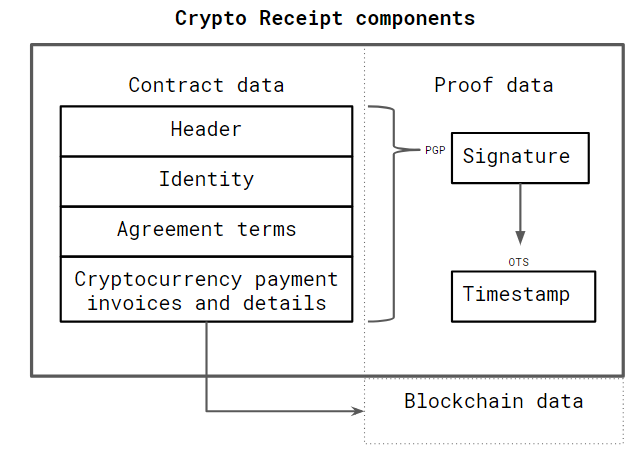
\includegraphics[width=\linewidth]{figures/cryptoreciepts_components.png}
\caption{Cryptoreciepts Components.\label{fig:components}}
\end{figure}


\subsubsection{Contract data}

The contract data consists of humanly readable text that can be encoded and parsed by software. It summarizes the contractual context of the transaction, including terms and conditions surrounding the payment and expected outcomes. More importantly, it also specifies the Bitcoin addresses to be used in the transaction, as well as the expected amounts and payment deadlines. 

Bitcoin payment request
Agreement, terms and contractual information
Identity of issuer

\begin{itemize}

\item \textbf{Bitcoin payment request}

\item \textbf{Agreement, terms and contractual information}

\item \textbf{Identity of issuer}

% TODO: these require more description of what they are

\end{itemize}


\subsubsection{Proof data}

The proof data consists of the cryptographic proofs that can be used to validate the claims of the parties to the contract. The cryptorecept protocol specifies the creation of two cryptographic proofs:

\begin{itemize}

\item \textbf{Digital signatures using PGP public-key cryptography}
\item \textbf{Trustless timestamps using Bitcoin as a notary}

% TODO: these require more description of what they are

\end{itemize}


\section{Bitcoin invoicing over the internet: Case-study of risks}
Users will request from Bylls that a certain amount of Canadian dollars be sent to a recipient. Bylls will present the user with an invoice request a specific amount of bitcoins be sent to a specific Bitcoin address generated uniquely for this invoice. The invoice also includes other payment terms such as the deadline at which the payment must be made for the exchange rate to be maintained, an industry standard practice to protect participants to an agreement from the volatility of the Bitcoin price. The user then sends the requested amount of bitcoins to Bylls’ Bitcoin address. Once confirmed in the Bitcoin blockchain, Bylls marks this invoice as paid and sends the funds to the recipient’s account provided to Bylls by the sender of the funds, and Bylls guarantees that the payment will be settled to the recipient within an agreed-upon timeframe.



\subsection{Man in the middle fraud}
The most serious risk associated with contracts and transactions settled in Bitcoin is security. Because Bitcoin transactions are irreversible, and bitcoins are liquid bearer assets that can be cashed out anonymously, they are a high value and high yield target for fraudster and thieves. The primary risk is a man-in-the-middle attack. This refers to a third party secretly obtaining, relaying or altering information during a transaction. In the overwhelming majority of cases, the attacker is trying to trick the payor of a transaction to send bitcoins to the attacker’s bitcoin address instead of the legitimate recipient. 

Dispute mediation in this case is extremely difficult since any investigation requires not only cooperation by both parties but also easily verifiable evidence. The burden of proof is often on the sender of the funds, since he is the aggrieved party that seeks restitution. Both senders and recipients have plausible deniability in most contexts, and the integrity and authenticity of evidence is always in question since it can be easily counterfeited. How can one prove that there was a covert third party that inserted himself and stole funds, and not some sort of internal fraud or elaborate scam?


\subsection{Phishing sites}
Fraudsters can impersonate online Bitcoin services and vendors using a technique called phishing, where they will try to convince users that they are dealing with a trusted service. Very often, phising attemps are performed via email where users receive invoices or by having websites with almost identical URL addresses (e.g. b7lls.com versus bylls.com). In the case of Bitcoin, the attacker can request a payment from the user, which believes he is dealing with a legitimate entity. In this case, the user can be lead to believe that he entered in agreement with another party who is completely unaware.  Bitcoin invoices sent by email are at an extremely high risk of phishing attack, which makes any invoicing system relying on email invoices without effective countermeasures such as Crypto Receipt a security risk and should be avoided.

Notably, the CEO of Bitcoin invoicing company Bitpay was himself the victim of a phishing scam\footnote{BitPay CEO Scammed for Over \$1.8 Million in Bitcoin \url{https://cointelegraph.com/news/bitpay-hacked-for-over-18-million-in-bitcoins}}, which demonstrates the need for higher cryptographic industry standards.


\subsection{Browser address replacement}
An attacker can hack the browser of the user, and remove Bylls’ Bitcoin address from the invoice page and replace it with his own address. In this case, the user will send the bitcoins to the hacker believing they are sending it to Bylls. Bylls will be unaware of this, and will simply believe that the payment hasn’t been sent and the invoice will expire. The user will not be able to prove that they sent the bitcoins to an address on the Bylls page. Again, in this scenario, Bylls has plausible deniability and the user would never be able to prove by himself that he was the victim of an attack (for example malware in a chrome extension) rather than Bylls defrauding him purposefully.


\subsection{Clipboard hijacking}
Clipboard hijacking is a man-in-the-middle fraud where a hacker will gain control of a user’s clipboard utility via malware. When the user copies the Bitcoin address from a website or sent to him via secure communications and pastes it in his Bitcoin wallet to send the bitcoins to the recipient, the malware will replace the address in the clipboard by his own, so that the sure can mistakenly send the bitcoins to the attacker.

In this case, dispute is also very difficult since the recipient has no way of knowing whether or not the claims of the sender are true, and perhaps the sender could believe that the website retroactively changed the address because he is unaware that he got hacker.


\section{Specifications}



\section{Crypto Receipt process}




\section{Conclusion}
